\section{Лабораторная работа 3 (вариант 5-8)}

\subsection{Задание}
Цель работы - создание программы, реализующей искусственный нейрон; разработка процедуры обучения нейрона; использование полученных результатов для решения тестовых задач классификации и аппроксимации.

\subsection{WTA нейрон}
Нейроны типа WTA (Winner Takes All — победитель получает все) всегда используются группами, в которых конкурируют между собой. Структурная схема группы (слоя) нейронов типа WTA представлена на рисунке ниже (рисунок \ref{img:wta}).

\begin{figure}[H]
\centering
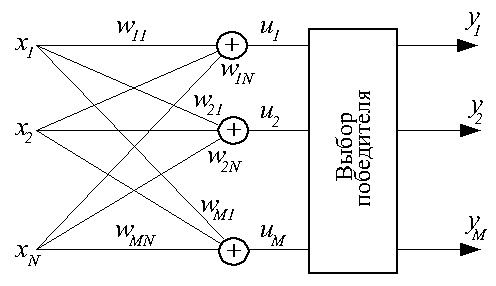
\includegraphics[scale=0.5]{wta.png}
\caption{Структурная схема слоя нейрона типа WTA}
\label{img:wta}
\end{figure}

Каждый конкурирующий нейрон в группе получает одни и те же входные сигналы. Каждый нейрон рассчитывает выходной сигнал своего сумматора обычным образом:

\begin{equation}\label{eq:Func}
	u_i=\sum\limits_{j=0}^N w_{ij} x_j.
\end{equation}

\begin{itemize}
\item По результатам сравнения всех $u_i, j=1, 2, ..., M$ выбирается нейрон-победитель, обладающий наибольшим значением $u_i$. Выходной сигнал $y_i$ нейрона-победителя получает значение 1, выходные сигналы всех остальных нейронов — 0.
\end{itemize}

Для обучения нейронов типа WTA не требуется учитель, оно практически полностью аналогично обучению инстара Гроссберга. Начальные значения весовых коэффициентов всех нейронов выбираются случайным образом с последующей нормализацией относительно 1.
При предъявлении каждого обучающего вектора $X^k$ определяется нейрон-победитель, что дает ему право уточнить свои весовые коэффициенты по упрощенному (в силу бинарности $y_i$) правилу Гроссберга:

\begin{equation}\label{eq:Func}
    w_{ij}(t+1)=w_{ij}(t)+\eta(x_j^k-w_{ij}(t)).
\end{equation}
Все проигравшие нейроны оставляют свои весовые коэффициенты неизменными. 

В каждом цикле обучения побеждает тот нейрон, чей текущий вектор входных весов $W_i$ наиболее близок входному вектору $X_k$. При этом вектор $W_i$ корректируется в сторону вектора $X_k$. Поэтому в ходе обучения каждая группа близких друг другу входных векторов (кластер) обслуживается отдельным нейроном.




Понятие «близости» двух векторов можно продемонстрировать на следующем примере. Пусть на очередной итерации обучения сети в режиме «онлайн» имеется входной вектор $X^k$. Тогда вычисление взвешенной суммы для i-го нейрона осуществляется по формуле:
\begin{equation}\label{eq:sum_func}
    u _ { i } = W _ { i } ^ { T } \cdot X ^ { k } = \sum _ { j = 1 } ^ { N } w _ { i j } \cdot x _ { j } ^ { k } = \left\| W _ { i } ^ { T } \right\| \cdot \left\| X ^ { k } \right\| \cdot \cos \left( \sphericalangle   W _ { i } , X ^ { k } \right)
\end{equation}

Поскольку вектора $W_i$ и $X^k$ нормализованы, то взвешенная сумма i-го нейрона равна косинусу угла между вектором весов и входным вектором. На рис. \ref{img:angle} представлена геометрическая интерпретация. Чем ближе весовой вектор ко входному, тем ближе косинус угла между векторами к 1.

\begin{figure}[H]
\centering
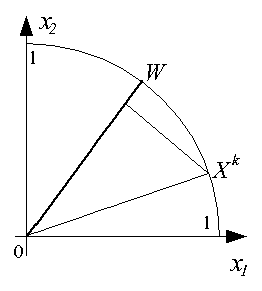
\includegraphics[scale=0.5]{angle.png}
\caption{Геометрическая интерпретация весов нейронов}
\label{img:angle}
\end{figure}

В режиме кластеризации при подаче на вход слоя нейронов типа WTA очередного вектора $X^k$ определяется степень его близости к векторам $W_i$ в виде косинусов углов между этими векторами, после чего определяется наиболее «близкий» вектор весов, отвечающий за тот или иной кластер.

Результат обучения слоя нейронов типа WTA на последовательности девяти двухкомпонентных входных векторов ${X^1, X^2, ..., X^9}$ иллюстрирует (рис. \ref{img:wta_teached}). Здесь были выделены три кластера входных векторов $\{X^1, X^8\}$, $\{X^3, X^4, X^5\}$ и $\{X^2, X^6, X^7, X^9\}$. За их распознавание отвечают три нейрона с векторами входных весов $W_1$, $W_2$ и $W_3$ соответственно.

\begin{figure}[H]
\centering
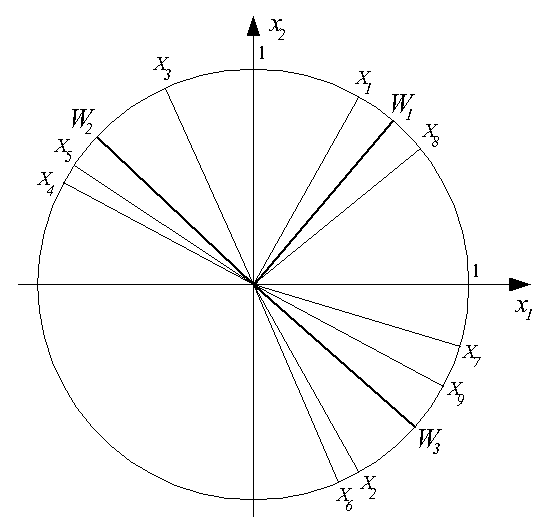
\includegraphics[scale=0.4]{wta_teached.png}
\caption{Результат обучения слоя нейронов типа WTA}
\label{img:wta_teached}
\end{figure}

Серьезная проблема в использовании нейронов типа WTA — возможность возникновения "мертвых" нейронов, т.е. нейронов, ни разу не победивших в конкурентной борьбе в ходе обучения и поэтому оставшихся в начальном состоянии. Для исключения "ложных" срабатываний в режиме классификации мертвые нейроны после окончания обучения должны быть удалены.

Для уменьшения количества мертвых нейронов (и, следовательно, повышения точности распознавания) используется модифицированное обучение, основанное на учете числа побед нейронов и шрафовании наиболее "зарвавшихся" среди них. Дисквалификация может быть реализована либо назначением порога числа побед, после которого слишком активный нейрон "засыпает" на заданное число циклов обучения, либо искусственным уменьшением величины  пропорционально числу побед.



\subsection{Исходные данные}

Обучающие данные для варианта 8 представлены на рисунке \ref{img:train_sphere}.

\begin{figure}[H]
\centering
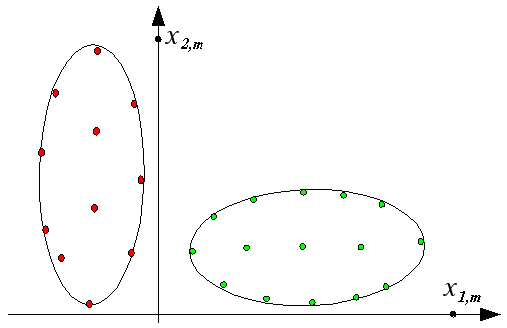
\includegraphics[scale=0.6]{train_sphere.png}
\caption{Данные для обучения варианта 8}
\label{img:train_sphere}
\end{figure}

\subsection{Обучение}

Для обучения были сгенерированы в случайном порядке точки, принадлежашие двум областям (рис. \ref{img:points}, а). После этого вектор входных значений, состоящих из координат точек, был нормализован (рис. \ref{img:points}, б) по формуле:
\begin{equation}\label{eq:normaFunc}
	x_{j}\leftarrow\frac{x_{j}}{\sqrt{x_{1}^{2}+x_{2}^{2}+\ldots+x_{N}^{2}}}.
\end{equation}

%\begin{figure}[h]
%    \begin{center}
%        \begin{minipage}[h]{0.48\linewidth}
%            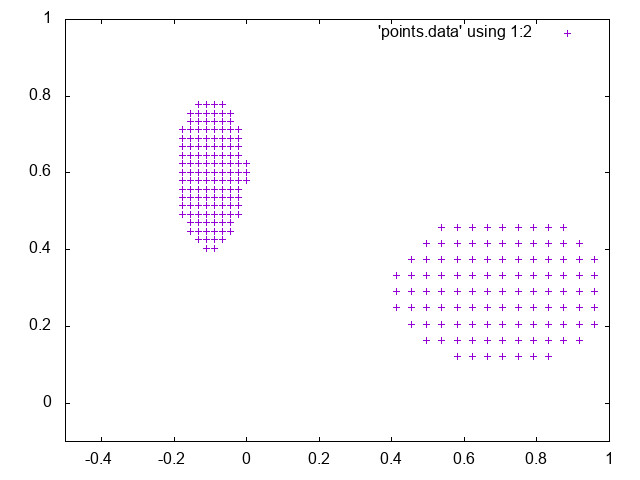
\includegraphics[width=1\linewidth]{points_nonorma.jpg}
%            %\caption{Обучающие данные} %% подпись к рисунку
%            \label{img:points} %% метка рисунка для ссылки на него
%        \end{minipage}
%        \hfill 
%        \begin{minipage}[h]{0.48\linewidth}
%            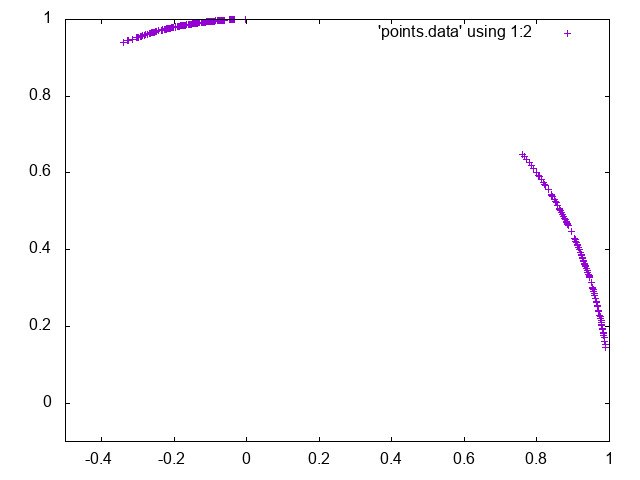
\includegraphics[width=1\linewidth]{points.png}
%            %\caption{Обчающие данные нормализованные}
%            \label{img:points_norma}
%        \end{minipage}
%        \begin{minipage}[h]{1\linewidth}
%            \centering
%            \begin{tabular}{p{0.50\linewidth}p{0.40\linewidth}}
%                %\centering % Обчающие данные после нормализации &
%                    \caption{Обучающие данные} &
%                %\centering %Обчающие данные после нормализации \\
%                    \caption{Обчающие данные после нормализации} \\
%            \end{tabular}
%        \end{minipage}
%    \end{center}
%\end{figure}


\begin{figure}[h]
    \begin{minipage}[h]{0.49\linewidth}
        \center{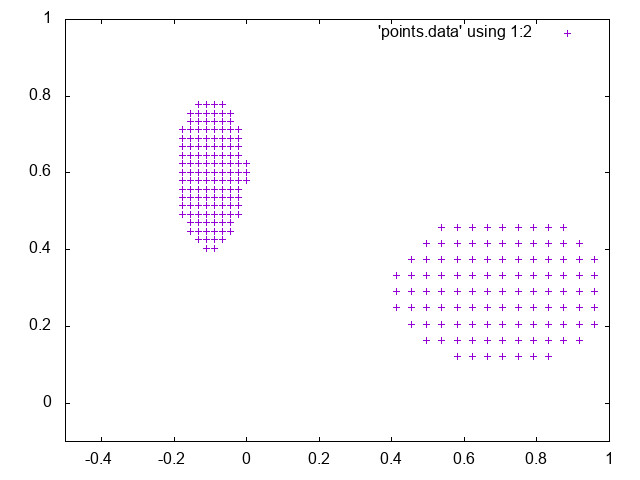
\includegraphics[width=1\linewidth]{points_nonorma.jpg} \\ а)}
    \end{minipage}
    \hfill
    \begin{minipage}[h]{0.49\linewidth}
        \center{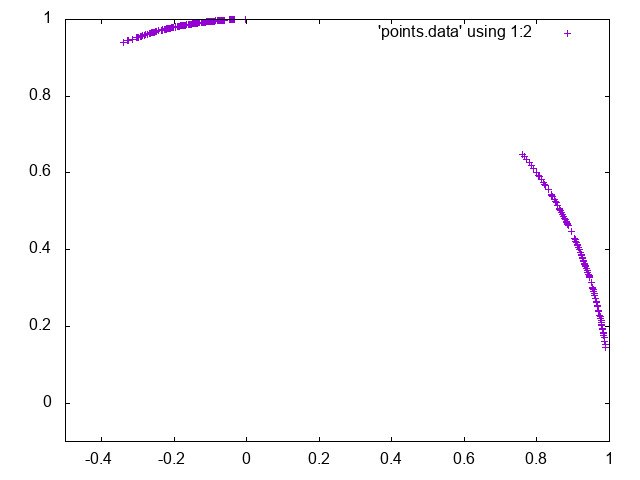
\includegraphics[width=1\linewidth]{points.png} \\ б)}
    \end{minipage}
    \caption{Обучающие данные}
    \label{img:points}
\end{figure}


Оба множнста имеют примерно одинаковое количесво точек. Это сделано, чтобы не допусть паревеса весов в сторону какого-либо из множеств.

Параметры обучения:
\begin{itemize}
    \item Размерность входных векторов: 2
    \item Количество нейронов: 4
    \item Количество эпох обучения: 2
    \item Коэффициент обучения $\eta$: 0,1
    \item Коэффициент штрафа при обучении: 0,01
    \item Начальные значения весов: (-1, -1) для всех весов
\end{itemize}

Обучение проводилось онлайн-методом - корректировка весов проводилась после подачи каджого входного вектора.

Коэффициент штрафа при обучении необходим для решения проблемы «мертвых» нейронов. Для каждого нейрона в слое вводится счетчик побед. Он изменяется на каждой итерации обучения для нейронов-победителей. Считчик используется для коррекции взвешенных сумм нейронов перед процедурой определения нейрона-победителя. Взвешенная сумма каждого нейрона рассчитывается по формуле:
\begin{equation}\label{eq:penaltyFunc}
    u _ { i } = \left( \sum _ { j = 1 } ^ { N } w _ { i j } \cdot x _ { j } \right) - p \cdot C_i,
\end{equation}
где $C_i, i=1, 2, ..., M$ - счетчик побед, p - коэффициент штрафа при обучении.

\subsection{Результат}

Результат процесса обучения представлен на рис. \ref{img:result}

\begin{figure}[h]
    \begin{minipage}[h]{0.49\linewidth}
        \center{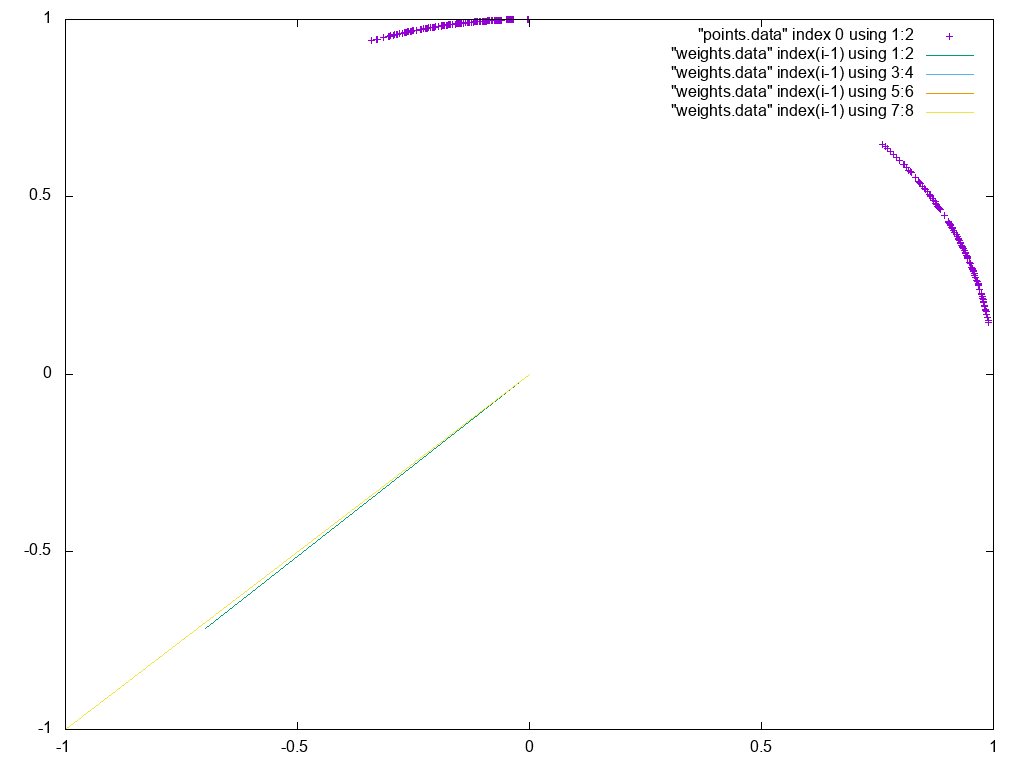
\includegraphics[width=1\linewidth]{train0.png} \\ а)}
    \end{minipage}
    \hfill
    \begin{minipage}[h]{0.49\linewidth}
        \center{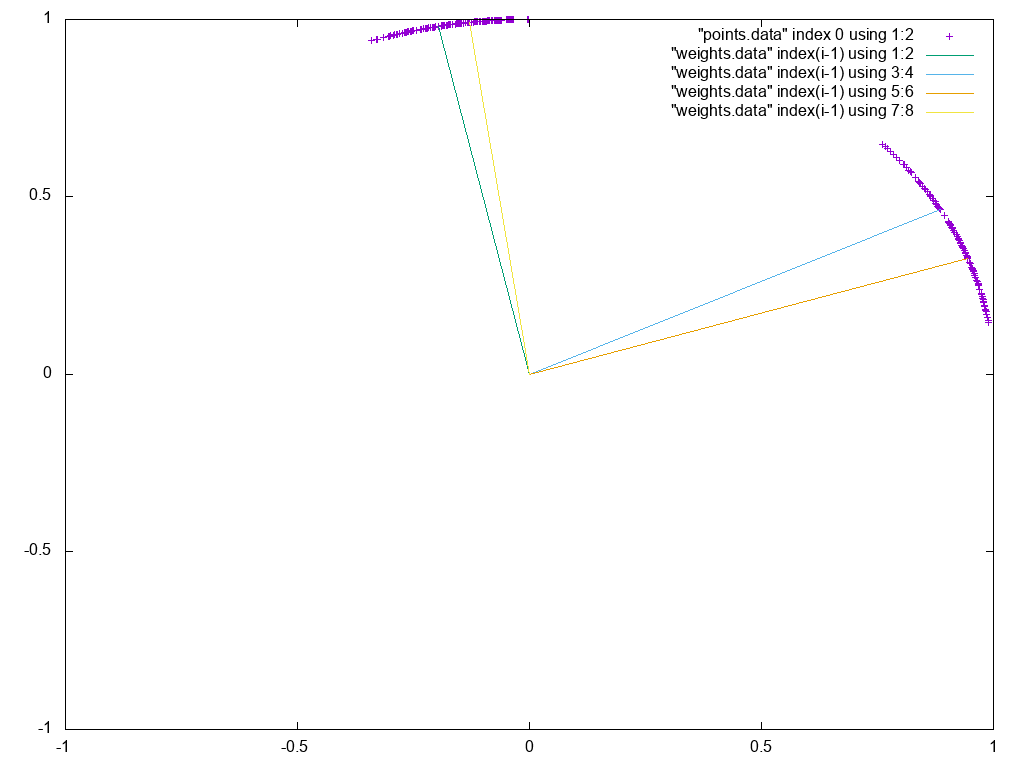
\includegraphics[width=1\linewidth]{train6.png} \\ б)}
    \end{minipage}
    \caption{a) - нулевое положение, б) - конечный результат}
    \label{img:result}
\end{figure}

Сам процесс обучения частично предствлен на рис. \ref{img:teaching}. Из начального положения $(x_1, x_2) = (-1, -1)$ (рис.\ref{img:teaching}, a), значения весов векторов  постепенно выравниваются и достигаю конечнго распределения, как на (рис.\ref{img:result}).

\begin{figure}[H]
    \begin{minipage}[h]{0.47\linewidth}
        \center{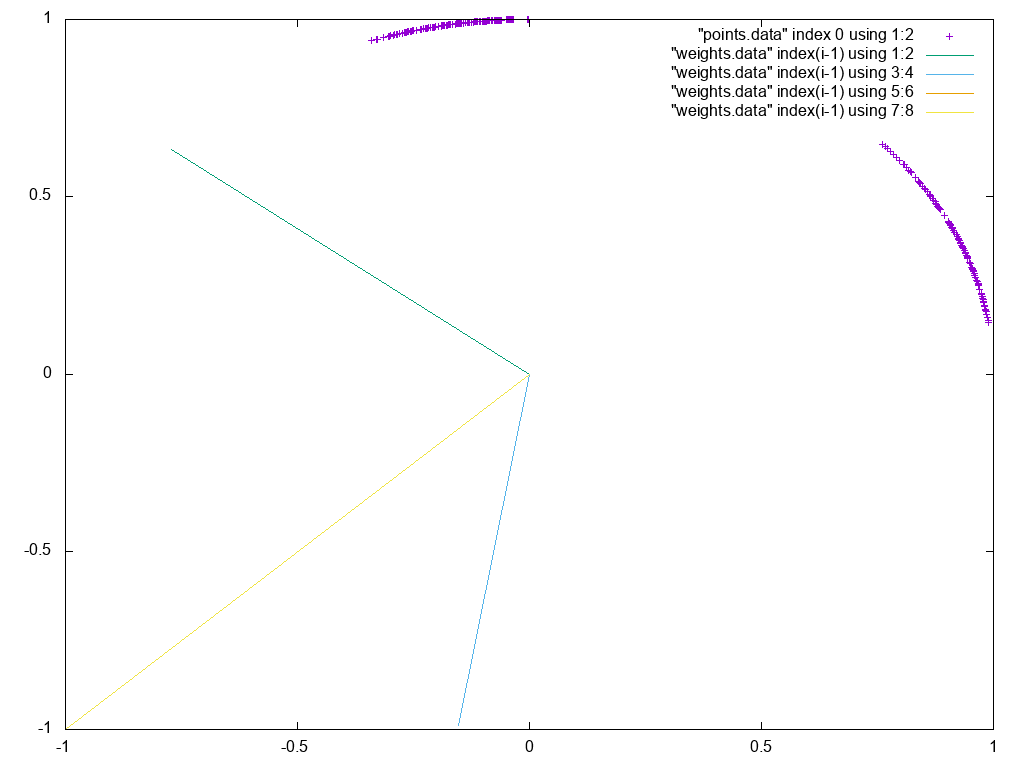
\includegraphics[width=1\linewidth]{train1.png} а)}  \\
    \end{minipage}
    \hfill
    \begin{minipage}[h]{0.47\linewidth}
        \center{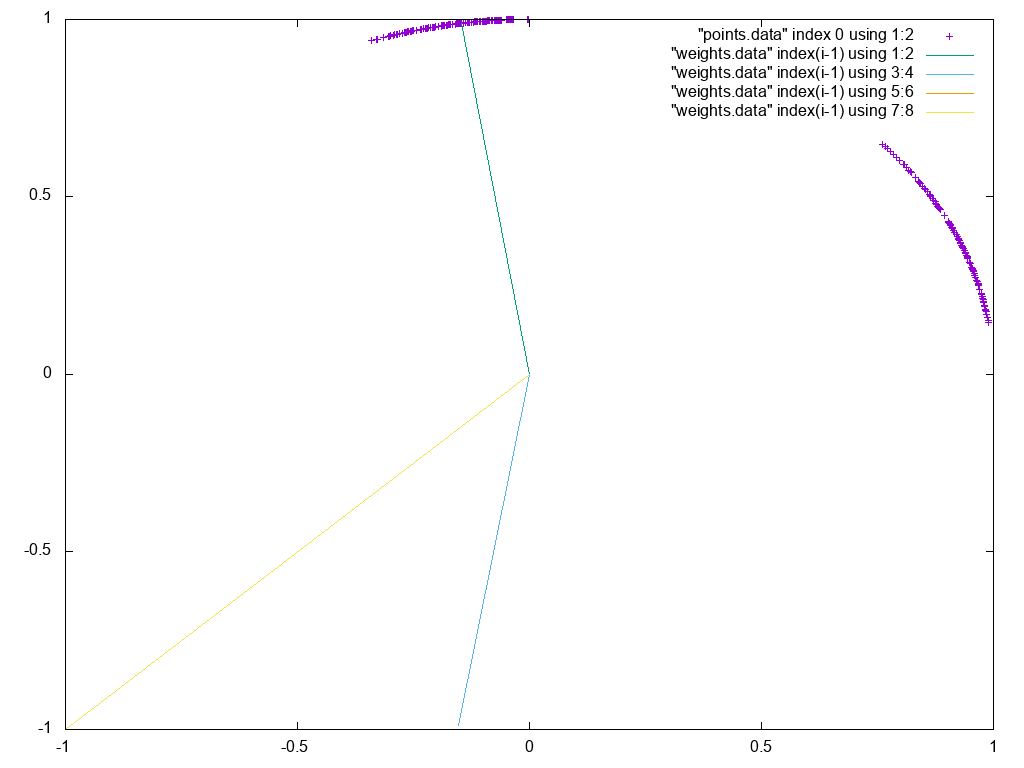
\includegraphics[width=1\linewidth]{train11.png} б)} \\
    \end{minipage}
    \vfill
    \begin{minipage}[h]{0.47\linewidth}
        \center{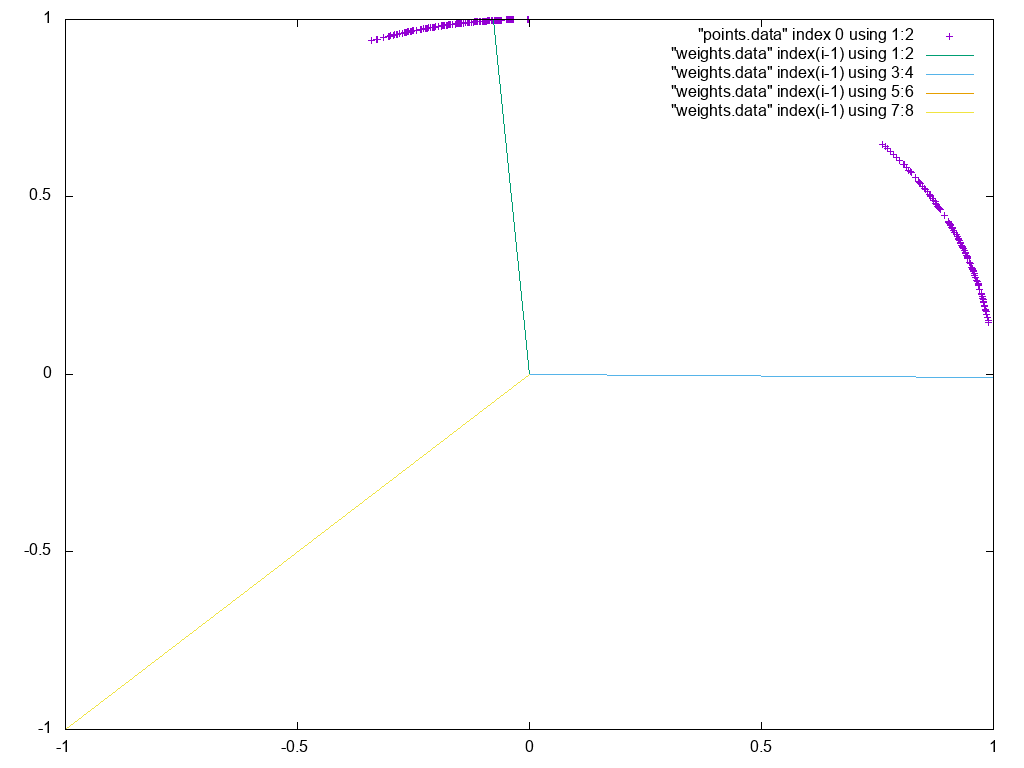
\includegraphics[width=1\linewidth]{train2.png} в)} \\
    \end{minipage}
    \hfill
    \begin{minipage}[h]{0.47\linewidth}
        \center{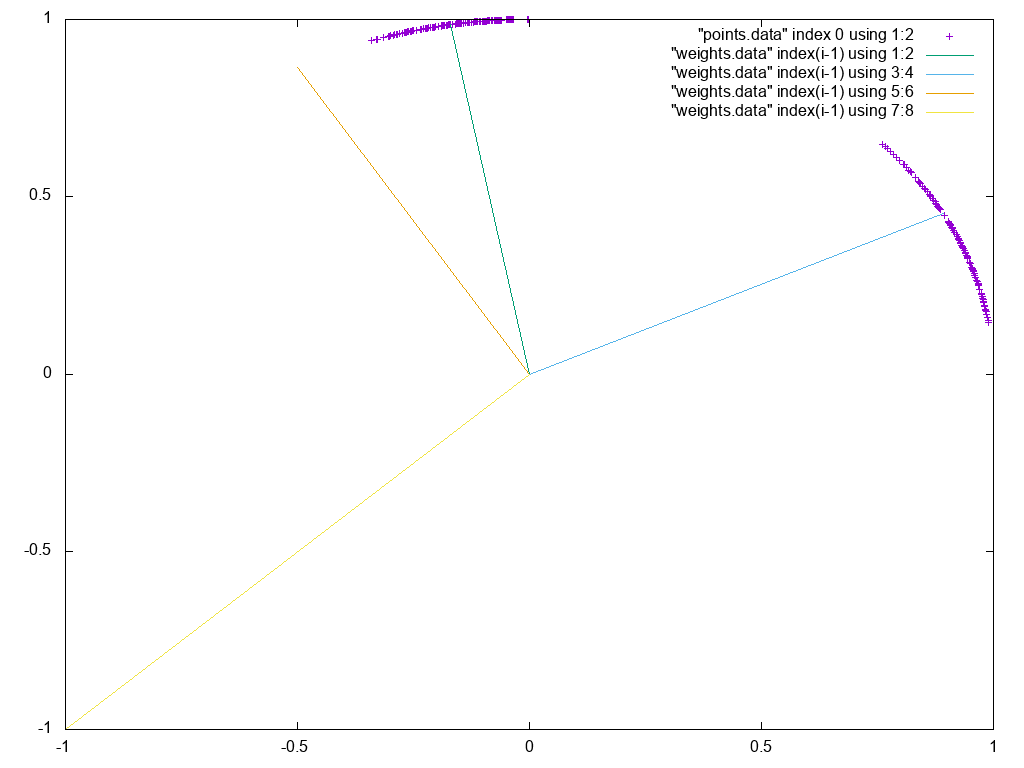
\includegraphics[width=1\linewidth]{train3.png} г)} \\
    \end{minipage}
    \vfill
    \begin{minipage}[h]{0.47\linewidth}
        \center{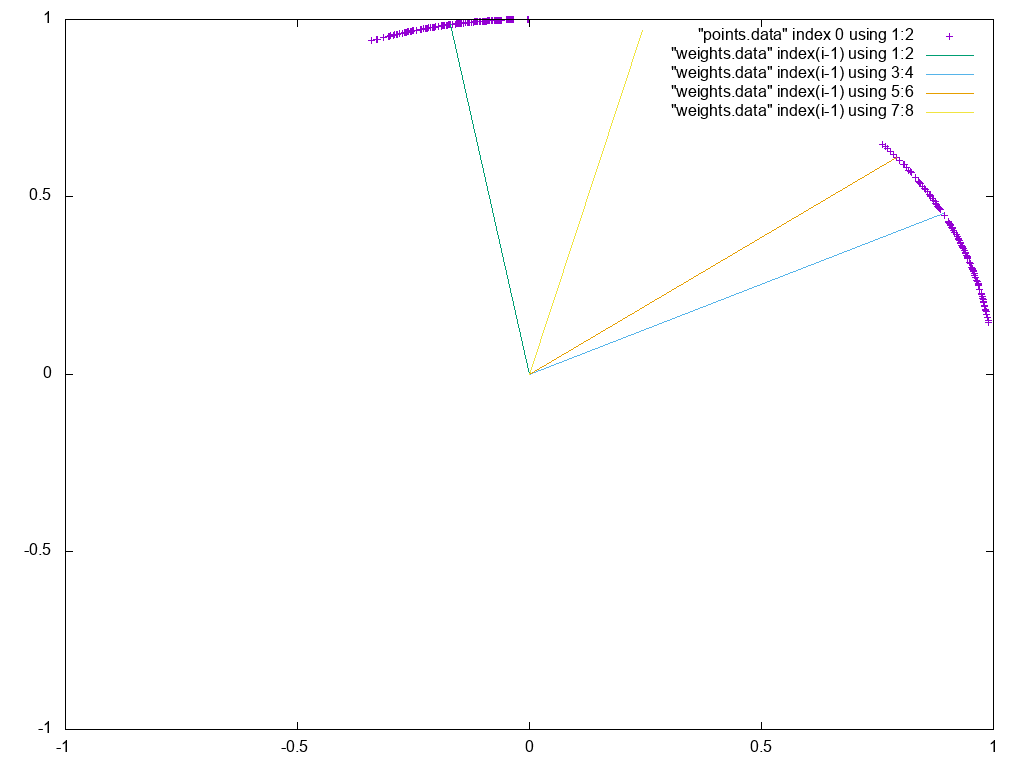
\includegraphics[width=1\linewidth]{train4.png} д)}  \\
    \end{minipage}
    \hfill
    \begin{minipage}[h]{0.47\linewidth}
        \center{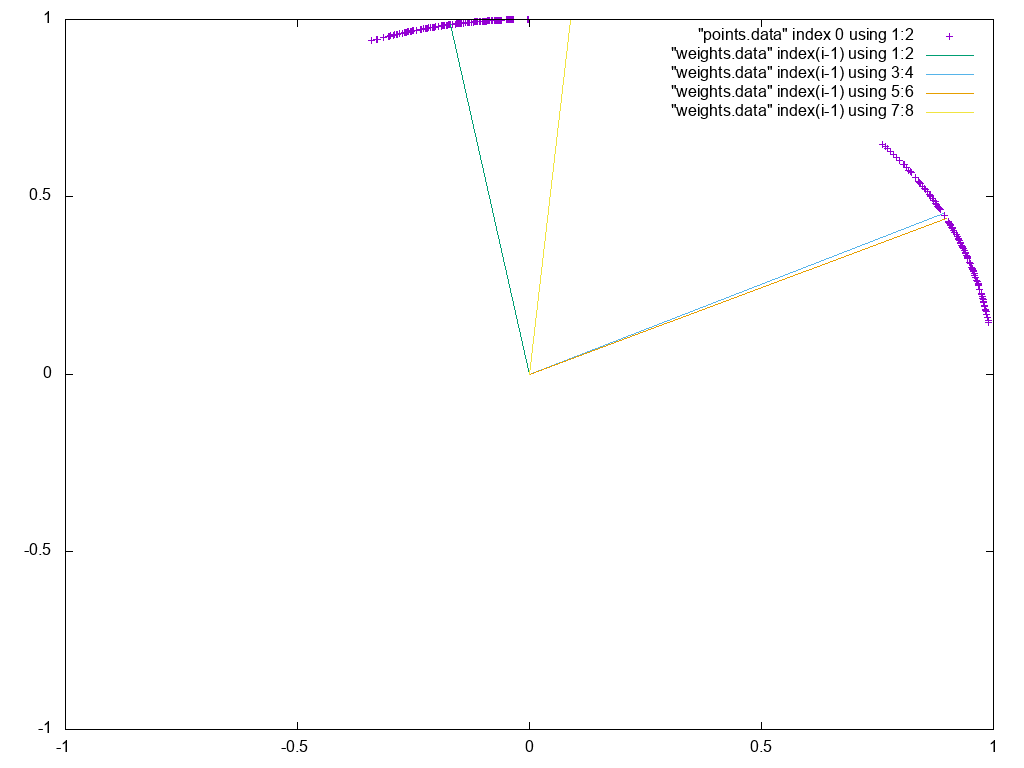
\includegraphics[width=1\linewidth]{train5.png} е)} \\
    \end{minipage}
    \caption{Процесс обучения}
    \label{img:teaching}
\end{figure}


\subsection{Иходный код}
Файл main.cpp
\begin{verbatim}

\end{verbatim}

Файл WTA.h
\begin{verbatim}
     
\end{verbatim}

Файл WTA.cpp
\begin{verbatim}
    
\end{verbatim}
